\section{Kết quả thí nghiệm}\label{sec:result}
\frame{\tableofcontents[currentsection]}

\begin{frame}{Kết quả thí nghiệm}
Tạo sinh cột mốc gương mặt trên tập GRID
\begin{figure}[H]
    \centering
    \includegraphics[width=15cm]{images/grid_examples-landmark.png}
    \caption{Kết quả tạo sinh cột mốc gương mặt theo giọng nói trên tập GRID}
\end{figure}
\end{frame}

\begin{frame}{Kết quả thí nghiệm}
Tạo sinh cột mốc gương mặt trên tập LRW
\begin{figure}[H]
    \centering
    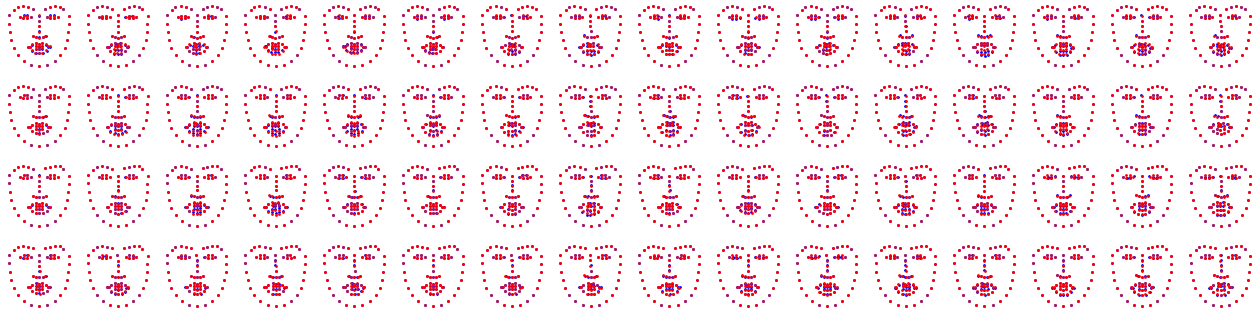
\includegraphics[width=15cm]{images/lrw_examples-landmark.png}
    \caption{Kết quả tạo sinh cột mốc gương mặt theo giọng nói trên tập LRW}
\end{figure}
\end{frame}

\begin{frame}{Kết quả thí nghiệm}
Tạo sinh gương mặt trên tập GRID
\begin{figure}[H]
    \centering
    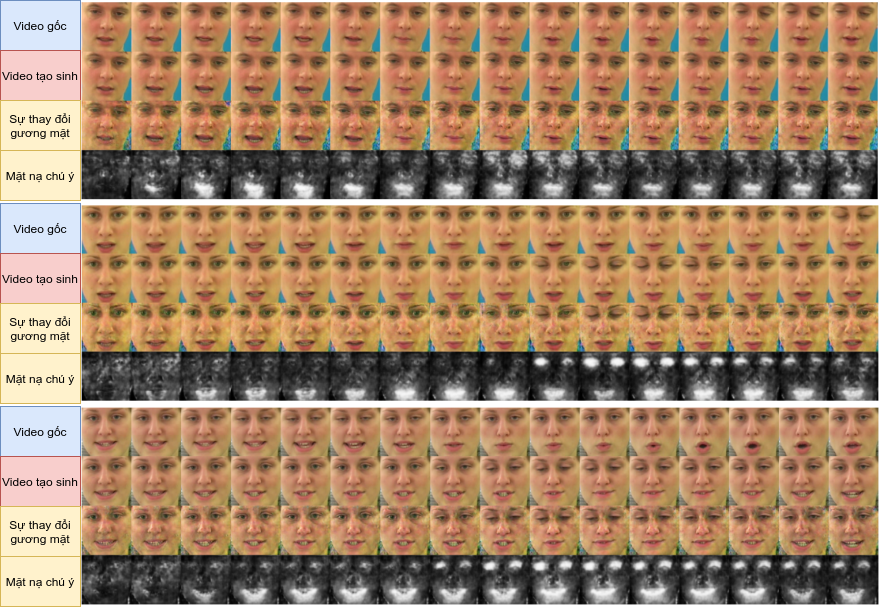
\includegraphics[width=9cm]{images/grid_examples-face.png}
    \caption{Kết quả tạo sinh gương mặt theo giọng nói trên tập GRID}
\end{figure}
\end{frame}

\begin{frame}{Kết quả thí nghiệm}
Tạo sinh gương mặt trên tập LRW
\begin{figure}[H]
    \centering
    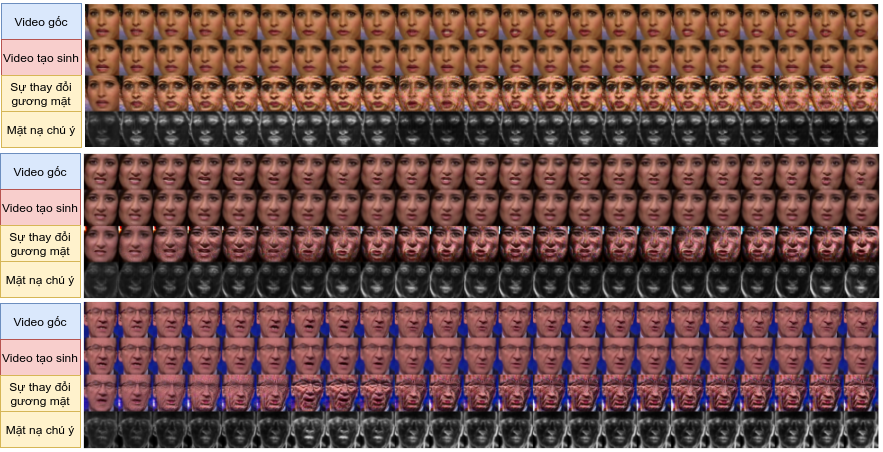
\includegraphics[width=12cm]{images/lrw_examples-frontal.png}
    \caption{Kết quả tạo sinh gương mặt theo giọng nói trên tập LRW}
\end{figure}
\end{frame}

\begin{frame}{Kết quả thí nghiệm}
\begin{table}[h]
    \centering
    \begin{tabular}{c | c | c | c | c}
    \hline 
    \multirow{2}{*}{\textbf{Phương pháp}} & \multicolumn{2}{c|}{\textbf{GRID}} & \multicolumn{2}{c}{\textbf{LRW}}\\
    \cline{2-5}
    & SSIM & CPBD & SSIM & CPBD\\
    \hline
    \textbf{Zakharov et al \cite{zakharov}} & 0.54 & 0.19 & 0.42 & 0.11 \\
    \textbf{Chung et al \cite{chung}} & 0.41 & \textbf{0.22} & 0.34 & \textbf{0.21} \\
    \textbf{Baseline (Chen et al) \cite{chen2019}} & 0.41 & 0.08 & 0.38 & 0.07 \\
    \hline
    \hline
    \textbf{Ours} & \textbf{0.72} & 0.12 & \textbf{0.54} & 0.06 \\
    \hline
    \end{tabular}
    \caption{So sánh với các mạng có cùng mục tiêu về độ đo SSIM và CPBD. Dữ liệu trong bảng được lấy từ bài khảo sát \cite{chen_survey}}
    \label{table:metrics_result}
\end{table}
\end{frame}

\begin{frame}{Kết quả thí nghiệm}
Tóm lại:
\begin{itemize}
    \item Luận văn đã chạy thử và kiểm chứng lại cấu trúc mạng của Lele Chen và cộng sự \cite{chen2020}
    \item Áp dụng có chỉnh sửa phương pháp chuẩn hóa cột mốc gương mặt từ bài báo \cite{gen_face_landmark} để cho ra kết quả tạo sinh hình ảnh tốt hơn so với bài báo gốc
    \item Chạy thử và đánh giá kết quả tạo sinh trên các dữ liệu khác bao gồm hình ảnh của người Việt và âm thanh tiếng Việt
\end{itemize}
\end{frame}
